\documentclass[11pt,a4paper]{article}
\usepackage[margin=2.1cm,top=2.5cm,headheight=26pt]{geometry}
\usepackage{amsmath,amssymb,bm}
\usepackage{siunitx}
\usepackage{booktabs}
\usepackage{graphicx}
\usepackage{tikz}
\usetikzlibrary{arrows.meta,calc,positioning,patterns}
\usepackage{pgfplots}
\pgfplotsset{compat=1.17}
\usepackage{enumitem}
\usepackage{float}
\usepackage{xcolor}
\usepackage{pifont}
\newcommand{\cmark}{\textcolor{green!45!black}{\ding{51}}}
\newcommand{\xmark}{\textcolor{red!70!black}{\ding{55}}}
\usepackage{fancyhdr}
\usepackage{tcolorbox}
\tcbuselibrary{skins,breakable}
\usepackage[colorlinks=true,linkcolor=blue!60!black,urlcolor=blue!60!black]{hyperref}
\sisetup{per-mode=symbol,detect-all}
\graphicspath{{figs/}}

\definecolor{navy}{RGB}{25,53,73}
\newtcolorbox{keybox}[1]{title={#1},colback=blue!4,colframe=blue!50!black,fonttitle=\bfseries,breakable}
\newtcolorbox{aerobox}[1]{title={#1},colback=orange!5,colframe=orange!60!black,fonttitle=\bfseries,breakable}
\newtcolorbox{sumbox}[1]{title={#1},colback=green!4,colframe=green!40!black,fonttitle=\bfseries,breakable}

% Photograph slot: renders the image if present in figs/, else a dashed placeholder.
\newcommand{\photo}[4]{%
  \begin{figure}[H]\centering
  \IfFileExists{figs/#1.jpg}{\includegraphics[width=#2\linewidth]{#1}}{%
  \IfFileExists{figs/#1.png}{\includegraphics[width=#2\linewidth]{#1}}{%
    \begin{tikzpicture}
      \draw[dashed,gray,line width=0.8pt] (0,0) rectangle (#2\linewidth,0.52*#2\linewidth);
      \node[align=center,text width=0.82*#2\linewidth,font=\footnotesize\itshape,gray!70!black]
        at (0.5*#2\linewidth,0.26*#2\linewidth) {PHOTOGRAPH: #4\\[3pt]\ttfamily figs/#1.jpg};
    \end{tikzpicture}}}
  \caption{#3}
  \end{figure}}

\pagestyle{fancy}
\fancyhf{}
\lhead{
\includegraphics[height=0.6cm]{logos/itu_logo_laci.pdf}\ \ UCK 364E Design of Machine Elements}
\rhead{Case Study 5 --- Handout}
\lfoot{\footnotesize Department of Aeronautical Engineering, Istanbul Technical University}
\rfoot{\footnotesize Page \thepage}

\begin{document}

\begin{center}
{\Large\textbf{Case Study: British Airways Flight 5390}}\\[3pt]
{\large\textbf{A margin of fifty belongs to the joint on the drawing, not to the joint that was built}}\\[5pt]
{\small Prof.\ Dr.\ Onur Tunçer \ $\cdot$\ UCK 364E Design of Machine Elements}
\end{center}

\vspace{2pt}\hrule\vspace{6pt}

\noindent\emph{Why you are reading this.} Lecture 6 taught you to check a tension joint three ways
--- against proof, against separation, against fatigue --- and Lecture 5 gave you the reason a nut
is as tall as it is: so that the bolt breaks before the thread strips. Both lectures assumed,
without saying so, that the bolt in the hole is the bolt on the drawing. This case study is a
tension joint with a static margin of more than fifty that failed on its first flight, because
that assumption was false in 84 of its 90 holes. The joint did not fail by bolt fracture. It
failed in the one mode nobody calculates for a correctly assembled joint: \textbf{the threads let
go.}

\section{What happened}

On \textbf{10 June 1990} a British Airways BAC One-Eleven 528FL, registration G-BJRT, left
Birmingham for Málaga as flight BA\,5390 with 81 passengers and six crew. At 07:33, climbing
through about \SI{17300}{ft} over Didcot, the left windscreen blew out of its frame. The commander
was drawn halfway out of the opening and was held there by cabin crew while the co-pilot flew the
aircraft to Southampton, landing at 07:55. Nobody died. The commander survived with fractures and
frostbite.

\medskip
The windscreen had been replaced during the night of 8--9 June, between about 03:00 and 05:00. The
accident flight, some 27 hours later, was the first since the change. A pressurised joint had been
built, signed for and released, and the first test it ever received was a climb with passengers on
board.

\begin{center}\small
\begin{tabular}{@{}ll@{}}
\toprule
Aircraft & BAC One-Eleven 528FL, G-BJRT, British Airways\\
Date, time & 10 June 1990, 07:33\\
Failure & left windscreen lost at about \SI{17300}{ft} pressure altitude\\
On board & 81 passengers, 4 cabin crew, 2 flight crew; no fatalities\\
Investigation & AAIB Aircraft Accident Report 1/92\\
\bottomrule
\end{tabular}
\end{center}

\section{The joint, and where the load goes}

\begin{figure}[H]\centering
\resizebox{0.92\textwidth}{!}{% Two ways to hold a windscreen: bolted on from outside (as built) and fitted as a plug from inside.
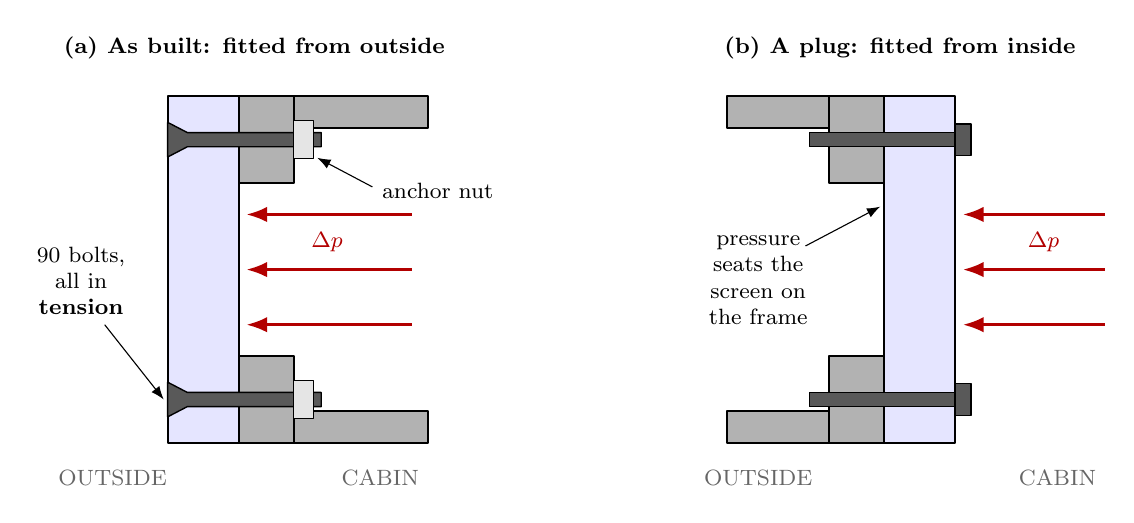
\begin{tikzpicture}[>=Latex,line join=round]
\tikzset{frm/.style={fill=black!30,draw=black,line width=0.7pt},
         scr/.style={fill=blue!10,draw=black,line width=0.7pt},
         blt/.style={fill=black!65,draw=black,line width=0.5pt},
         pr/.style={->,red!70!black,line width=1pt}, lab/.style={font=\footnotesize}}
% ---------- (a) as built ----------
\begin{scope}
  \node[lab,anchor=south] at (2.4,4.75) {\textbf{(a) As built: fitted from outside}};
  \node[lab,black!60] at (0.6,-0.45) {OUTSIDE}; \node[lab,black!60] at (4.0,-0.45) {CABIN};
  % frame (airframe) on the cabin side, top and bottom members
  \path[frm] (2.2,4.4) rectangle (2.9,3.3); \path[frm] (2.2,1.1) rectangle (2.9,0);
  \path[frm] (2.9,4.4) rectangle (4.6,4.0); \path[frm] (2.9,0.4) rectangle (4.6,0);
  % windscreen on the outside face of the frame
  \path[scr] (1.3,4.4) rectangle (2.2,0);
  % bolts: countersunk heads outside, anchor nuts inside
  \foreach \y in {3.85,0.55}{
    \path[blt] (1.3,\y+0.22) -- (1.55,\y+0.09) -- (3.25,\y+0.09) -- (3.25,\y-0.09) -- (1.55,\y-0.09) -- (1.3,\y-0.22) -- cycle;
    \path[fill=black!10,draw=black,line width=0.5pt] (2.9,\y+0.24) rectangle (3.15,\y-0.24);}
  \foreach \y in {1.5,2.2,2.9}{\draw[pr] (4.4,\y) -- (2.3,\y);}
  \node[lab,text=red!70!black,anchor=west] at (3.0,2.55) {$\Delta p$};
  \draw[<-,line width=0.4pt] (3.2,3.62) -- (3.9,3.25); \node[lab,anchor=west] at (3.9,3.2) {anchor nut};
  \draw[<-,line width=0.4pt] (1.25,0.55) -- (0.5,1.5); \node[lab,anchor=south,align=center] at (0.2,1.5) {90 bolts,\\ all in\\ \textbf{tension}};\node[lab,anchor=south] at (1.75,-0.02) {};
\end{scope}
% ---------- (b) plug ----------
\begin{scope}[xshift=8.2cm]
  \node[lab,anchor=south] at (2.4,4.75) {\textbf{(b) A plug: fitted from inside}};
  \node[lab,black!60] at (0.6,-0.45) {OUTSIDE}; \node[lab,black!60] at (4.4,-0.45) {CABIN};
  \path[frm] (1.5,4.4) rectangle (2.2,3.3); \path[frm] (1.5,1.1) rectangle (2.2,0);
  \path[frm] (0.2,4.4) rectangle (1.5,4.0); \path[frm] (0.2,0.4) rectangle (1.5,0);
  \path[scr] (2.2,4.4) rectangle (3.1,0);
  \foreach \y in {3.85,0.55}{\path[blt] (1.25,\y+0.09) rectangle (3.2,\y-0.09); \path[blt] (3.1,\y+0.2) rectangle (3.3,\y-0.2);}
  \foreach \y in {1.5,2.2,2.9}{\draw[pr] (5.0,\y) -- (3.2,\y);}
  \node[lab,text=red!70!black,anchor=west] at (3.9,2.55) {$\Delta p$};
  \draw[<-,line width=0.4pt] (2.15,3.0) -- (1.2,2.5); \node[lab,anchor=north,align=center] at (0.6,2.75) {pressure\\ seats the\\ screen on\\ the frame};
\end{scope}
\end{tikzpicture}
}
\caption{Two ways to hold a windscreen. In (a), as on this aircraft, cabin pressure tries to push
the screen off the frame and every bolt is in tension. In (b) the same pressure presses the screen
onto the frame; the fasteners locate it and seal it, and a wrong fastener is an inconvenience
instead of an accident.}
\label{fig:joint}
\end{figure}

The One-Eleven windscreen is fitted \emph{from the outside} of the aircraft and held by
\textbf{90 countersunk bolts}, also fitted from outside, which screw into 10 UNF floating
self-locking anchor nuts on the frame (AAIB 1.6.3). That makes it a tension joint in the sense of
Lecture 6: the pressure load goes through the bolt threads and nowhere else.

\medskip
The report makes a point that matters for everything that follows. Ninety bolts are there
\emph{to seal}, not to carry load: ``the large number of bolts are required to prevent leakage of
pressurised air through the window seal, but the force of internal air pressure could be
satisfactorily resisted by far fewer bolts.'' The joint is enormously over-strength in bolt
tension. We will put a number on that in \S\ref{sec:arith}.

\section{Three bolts that look alike}

\begin{center}\small
\begin{tabular}{@{}lllll@{}}
\toprule
Part number & Thread & Shank length & Measured diameter & Fitted on 9 June\\
\midrule
A211-8D \ (specified) & 10-32 UNF & \SI{0.8}{in} & 0.1865--\SI{0.1895}{in} & \textbf{0}\\
A211-8C & 8-32 UNC & \SI{0.8}{in} & 0.1605--\SI{0.1639}{in} & \textbf{84}\\
A211-7D & 10-32 UNF & \SI{0.7}{in} & as 8D & \textbf{6}\\
\bottomrule
\end{tabular}
\end{center}

\noindent Not one of the ninety was the specified bolt (AAIB 1.12.1). Eighty-four were the right
length and \SI{0.026}{in} too thin; six were the right diameter and \SI{0.1}{in} too short.

\medskip
There is a second error underneath the first. The \emph{old} windscreen, fitted about four years
earlier, had itself been held mostly by the short A211-7D bolts: 78 of the 80 recovered. So when
the engineer matched new bolts against an old one, his reference was already wrong. An error that
does no visible harm becomes the standard the next person copies.

\subsection*{Why the wrong bolt goes in, and feels right}

No.\,10 and No.\,8 threads in these series have the \textbf{same pitch}: 32 threads per inch. An
8-32 bolt therefore runs freely into a 10-32 nut --- the helices match --- and only the diameters
differ. With $p=1/32=\SI{0.03125}{in}$, the Unified thread relations give
\[
d_2 = d-0.6495\,p,\qquad D_1 = D-1.0825\,p,\qquad A_t=\frac{\pi}{4}\left(d-0.9743\,p\right)^2 .
\]

\begin{center}\small
\begin{tabular}{@{}lcc@{}}
\toprule
 & 10-32 UNF & 8-32 UNC\\
\midrule
Major diameter $d$, in & 0.1900 & 0.1640\\
Pitch diameter $d_2$, in & 0.1697 & 0.1437\\
Nut minor diameter $D_1$, in & 0.1562 \ (class 2B: 0.156--0.164) & ---\\
Tensile stress area $A_t$, in$^2$ & 0.0200 & 0.0140\\
\bottomrule
\end{tabular}
\end{center}

What holds a bolt in a nut is the radial overlap of the two thread forms --- half the difference
between the bolt's major diameter and the nut's minor diameter:
\[
e=\tfrac12\left(d_{\text{bolt}}-D_{1,\text{nut}}\right).
\]

\begin{center}\small
\begin{tabular}{@{}lll@{}}
\toprule
Pair & Overlap $e$ & Share of full depth\\
\midrule
10-32 bolt in 10-32 nut & $(0.1900-0.1562)/2=\SI{0.0169}{in}$ & \SI{100}{\percent}\\
8-32 bolt in 10-32 nut, best case & $(0.1639-0.1562)/2=\SI{0.0039}{in}$ & \SI{23}{\percent}\\
8-32 bolt in 10-32 nut, worst case & $(0.1605-0.1640)/2<0$ & \textbf{none}\\
\bottomrule
\end{tabular}
\end{center}

\begin{figure}[H]\centering
\resizebox{\textwidth}{!}{% Thread engagement to scale: 1 mm on the page = 0.001 in.  10-32 UNF nut; (a) 10-32 bolt, (b) 8-32 bolt.
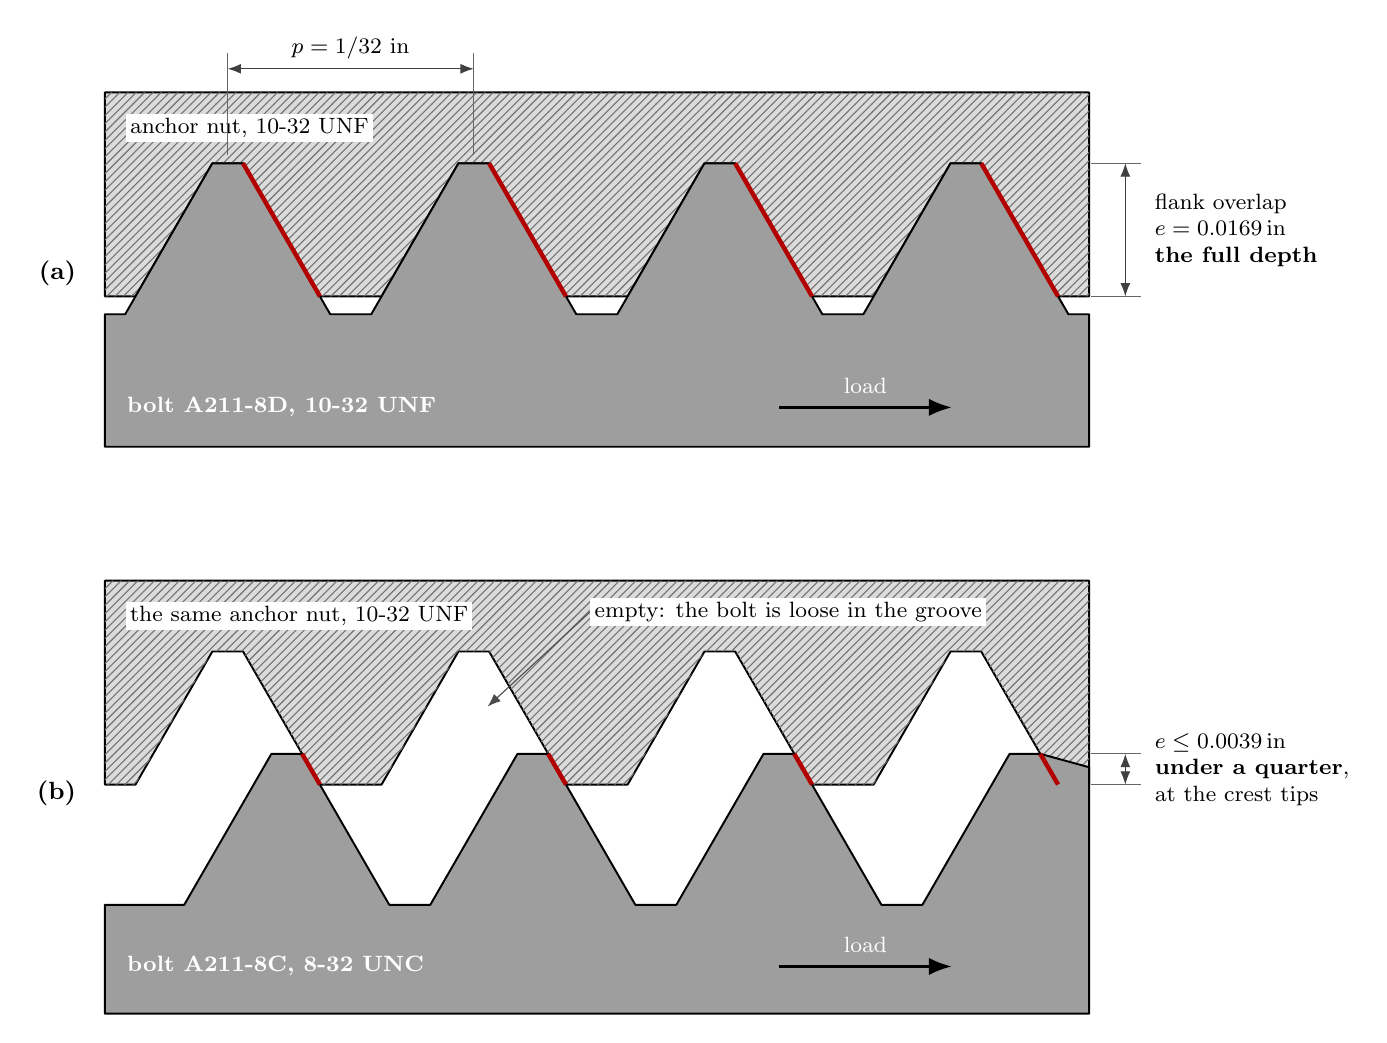
\begin{tikzpicture}[x=1mm,y=1mm,>=Latex,line join=round]
\tikzset{nut/.style={fill=black!14,draw=black,line width=0.7pt},
         nuth/.style={pattern=north east lines,pattern color=black!55},
         blt/.style={fill=black!38,draw=black,line width=0.7pt},
         dimn/.style={<->,black!75,line width=0.4pt}, lab/.style={font=\footnotesize}}
\def\p{31.25}
% ---- nut profile (same in both panels): grooves centred at x = k p ; radii in mil, drawn at y = r - 55
\newcommand{\nutprofile}[1]{% #1 = y offset
  \begin{scope}[yshift=#1]
  \path[nut] (-15.6,49) -- (-15.6,23.1) -- (-11.71,23.1) -- (-1.95,40) -- (1.95,40) -- (11.71,23.1)
    \foreach \k in {1,2,3}{ -- ({\k*\p-11.71},23.1) -- ({\k*\p-1.95},40) -- ({\k*\p+1.95},40) -- ({\k*\p+11.71},23.1)}
    -- (109.4,23.1) -- (109.4,49) -- cycle;
  \path[nuth] (-15.6,49) -- (-15.6,23.1) -- (-11.71,23.1) -- (-1.95,40) -- (1.95,40) -- (11.71,23.1)
    \foreach \k in {1,2,3}{ -- ({\k*\p-11.71},23.1) -- ({\k*\p-1.95},40) -- ({\k*\p+1.95},40) -- ({\k*\p+11.71},23.1)}
    -- (109.4,23.1) -- (109.4,49) -- cycle;
  \end{scope}}

% ================= (a) correct bolt =================
\nutprofile{0mm}
\path[blt] (-15.6,4) -- (-15.6,20.83) -- (-13.02,20.83) -- (-1.95,40) -- (1.95,40) -- (13.02,20.83)
  \foreach \k in {1,2,3}{ -- ({\k*\p-13.02},20.83) -- ({\k*\p-1.95},40) -- ({\k*\p+1.95},40) -- ({\k*\p+13.02},20.83)}
  -- (109.4,20.83) -- (109.4,4) -- cycle;
\foreach \k in {0,1,2,3}{\draw[red!70!black,line width=1.6pt] ({\k*\p+11.71},23.1) -- ({\k*\p+1.95},40);}
\node[lab,anchor=west,fill=white,inner sep=1.5pt] at (-13,44.5) {anchor nut, 10-32 UNF};
\node[lab,anchor=west,text=white] at (-14,9) {\textbf{bolt A211-8D, 10-32 UNF}};
\draw[dimn] (114,23.1) -- (114,40); \draw[black!60,line width=0.3pt] (109.6,23.1) -- (116,23.1) (109.6,40) -- (116,40);
\node[lab,anchor=west,align=left] at (116.5,31.5) {flank overlap\\ $e=\SI{0.0169}{in}$\\ \textbf{the full depth}};
\draw[dimn] (0,52) -- (\p,52); \draw[black!60,line width=0.3pt] (0,41) -- (0,54) (\p,41) -- (\p,54);
\node[lab,anchor=south] at (15.6,52) {$p=1/32$ in};
\draw[->,line width=1.2pt] (70,9) -- (92,9); \node[lab,anchor=south,text=white] at (81,9.5) {load};
\node[font=\small\bfseries,anchor=east] at (-18,26) {(a)};

% ================= (b) wrong bolt, shifted axially onto its loaded flanks =================
\begin{scope}[yshift=-62mm]
\nutprofile{0mm}
% 8-32 bolt: pitch radius 71.85, major 82, minor 62.83 ; drawn shifted by +7.5 so the right-hand flanks touch
\path[blt] (-15.6,-6) -- (-15.6,7.83) -- (-5.52,7.83) -- (5.55,27) -- (9.45,27) -- (20.52,7.83)
  \foreach \k in {1,2}{ -- ({\k*\p+7.5-13.02},7.83) -- ({\k*\p+7.5-1.95},27) -- ({\k*\p+7.5+1.95},27) -- ({\k*\p+7.5+13.02},7.83)}
  -- ({3*\p+7.5-13.02},7.83) -- ({3*\p+7.5-1.95},27) -- ({3*\p+7.5+1.95},27) -- (109.4,25.3) -- (109.4,-6) -- cycle;
\foreach \k in {0,1,2,3}{\draw[red!70!black,line width=1.6pt] ({\k*\p+11.71},23.1) -- ({\k*\p+9.45},27);}
\node[lab,anchor=west,fill=white,inner sep=1.5pt] at (-13,44.5) {the same anchor nut, 10-32 UNF};
\node[lab,anchor=west,text=white] at (-14,0) {\textbf{bolt A211-8C, 8-32 UNC}};
\draw[dimn] (114,23.1) -- (114,27); \draw[black!60,line width=0.3pt] (109.6,23.1) -- (116,23.1) (109.6,27) -- (116,27);
\node[lab,anchor=west,align=left] at (116.5,25) {$e\le\SI{0.0039}{in}$\\ \textbf{under a quarter},\\ at the crest tips};
\draw[->,line width=1.2pt] (70,0) -- (92,0); \node[lab,anchor=south,text=white] at (81,0.5) {load};
\draw[<-,black!70,line width=0.4pt] (33,33) -- (46,45); \node[lab,anchor=west,fill=white,inner sep=1.5pt] at (46,45) {empty: the bolt is loose in the groove};
\node[font=\small\bfseries,anchor=east] at (-18,22) {(b)};
\end{scope}
\end{tikzpicture}
}
\caption{The two engagements, drawn to scale from the basic thread dimensions. The red lines are the loaded flanks actually in contact. In (b) the bolt
has been slid along until its flanks touch: it carries load on a band less than four thousandths
of an inch wide, at the very tips of both thread forms.}
\label{fig:thread}
\end{figure}

Depending on where each bolt and each nut fell in its tolerance band, the wrong bolt engaged
somewhere between a quarter of the thread depth and nothing at all. That the bolts held at all owes
something to the nuts being the self-locking kind, whose deformed threads grip a bolt that a plain
nut of the same size would let slide through.

\section{The arithmetic, in the symbols of Lectures 5 and 6}
\label{sec:arith}

\begin{aerobox}{Assumptions --- these are \emph{not} from the report}
The investigation did not publish a load calculation, so the demand side is estimated here. Change
the numbers and repeat the working; the conclusion does not move.

\smallskip
{\small
\begin{tabular}{@{}lll@{}}
Cabin differential at \SI{17300}{ft} & \SI{34.5}{kPa} (\SI{5}{psi}) & estimate; the maximum is \SI{7.5}{psi} (AAIB 1.6.3)\\
Windscreen pressure area & \SI{0.5}{m^2} (\SI{775}{in^2}) & estimate: 90 bolts at about \SI{1.3}{in} pitch\\
Bolt ultimate strength $S_{ut}$ & \SI{860}{MPa} (\SI{125}{ksi}) & typical aircraft steel bolt\\
Engaged length $L_e$ & 5 threads $=\SI{0.156}{in}$ & about five threads show through the nut\\
Nut factor $K$ & 0.20 & Lecture 5 default, dry\\
\end{tabular}}
\end{aerobox}

\subsection*{Step 1 --- the demand}
\[
F_{\text{total}}=\Delta p\,A=5\times775\approx\SI{3900}{lbf}\ (\SI{17}{kN}),\qquad
P=\frac{3900}{90}\approx\SI{43}{lbf}\ (\SI{0.19}{kN})\ \text{per bolt}.
\]
Forty-three pounds on a No.\,10 bolt. At the full \SI{7.5}{psi} it is \SI{65}{lbf}
(\SI{0.29}{kN}). This is what ``far fewer bolts'' means.

\subsection*{Step 2 --- the correct bolt in tension}
\[
P_t=A_t\,S_{ut}=0.0200\times\num{125000}=\SI{2500}{lbf}\ (\SI{11.1}{kN}),\qquad n=\frac{2500}{43}\approx\mathbf{58}.
\]
And the joint would never have separated. At the specified \SI{15}{lbf.in} the preload is
$F_i=T/(Kd)=15/(0.20\times0.190)\approx\SI{395}{lbf}$ (\SI{1.8}{kN}), nine times the external
load before the joint constant $C$ is even applied.

\subsection*{Step 3 --- thread strip, correct pair}
The shear area of the external thread, taken at the nut's minor diameter (the FED-STD-H28 form),
for $n$ threads per inch:
\[
A_s=\pi\,n\,L_e\,D_1\left[\frac{1}{2n}+0.577\left(d_2-D_1\right)\right]
\]
\[
A_s=\pi(32)(0.156)(0.1562)\left[0.01563+0.577(0.1697-0.1562)\right]=\SI{0.0574}{in^2}
\]
\[
P_s=0.577\,S_{ut}\,A_s=0.577\times\num{125000}\times0.0574\approx\SI{4100}{lbf}\ (\SI{18}{kN})\ >\ P_t .
\]
The strip area is 2.9 times $A_t$. \textbf{The bolt breaks before the thread strips} --- the order
Lecture 5 said a sound joint must have. Notice which quantity that order hangs on: the bracket
contains $d_2-D_1$, the fit between \emph{this} bolt and \emph{this} nut. It is a property of the
pair, not of the bolt.

\subsection*{Step 4 --- thread strip, wrong pair}
Put the 8-32 pitch diameter into the same formula:
\[
A_s=\pi(32)(0.156)(0.1562)\left[0.01563+0.577(0.1437-0.1562)\right]=\SI{0.0206}{in^2}.
\]
That is \SI{36}{\percent} of the correct value and suggests about \SI{1500}{lbf} per bolt --- a
margin of 35. \textbf{Do not believe it.} The formula assumes flanks that are supported over their
full depth and shear cleanly on a cylinder. Figure~\ref{fig:thread}(b) shows what is actually
there:
\begin{itemize}[leftmargin=*,itemsep=1pt]
\item contact is confined to the outer \SI{0.004}{in} of the flanks at best, and crest rounding
  removes part of that;
\item the \ang{60} flanks turn the axial load into a radial force $F\tan\ang{30}$ that pushes the
  two thread forms apart;
\item the floating nut lets the bolt sit off-centre, so one side carries and the other does not;
\item the failure is crushing of the crest tips and ride-over, not shear on a cylinder.
\end{itemize}
A formula is only as good as the failure mode it was derived for. When the geometry leaves the
range the formula assumed, the right move is to stop calculating and test.

\subsection*{Step 5 --- what the tests found}
The AAIB did test (1.16.1). They wound 8 UNC bolts into 10 UNF anchor nuts --- twenty on the
bench, thirty-two on an aircraft, ten into G-BJRT's own nuts --- and recorded the torque at which
the threads slipped: between \textbf{zero and \SI{12}{lbf.in}}, \textbf{\SI{4.7}{lbf.in} on
average}. Convert with the torque--preload relation of Lecture 5, $T=K\,d\,F$:
\[
F=\frac{T}{K\,d}=\frac{4.7}{0.20\times0.164}\approx\SI{140}{lbf}\ (\SI{0.64}{kN}),\qquad
F_{\max}=\frac{12}{0.20\times0.164}\approx\SI{370}{lbf}\ (\SI{1.6}{kN}).
\]
These are upper bounds: the anchor nuts are self-locking, so part of that torque was prevailing
friction and never became axial force.

\medskip
Now compare with what was done on the night. The manual called for \SI{15}{lbf.in}. The engineer
used a torque-limiting screwdriver set to \SI{20}{lbf.in} (1.17.4). \textbf{Twenty is above every
slip torque the investigation ever measured.} Many of the joints must have slipped while they were
being tightened, leaving flattened crests and little or no preload --- and a slipping thread and a
releasing clutch feel much the same in the hand.

\begin{figure}[H]\centering
% Capacity and demand per bolt, log scale.
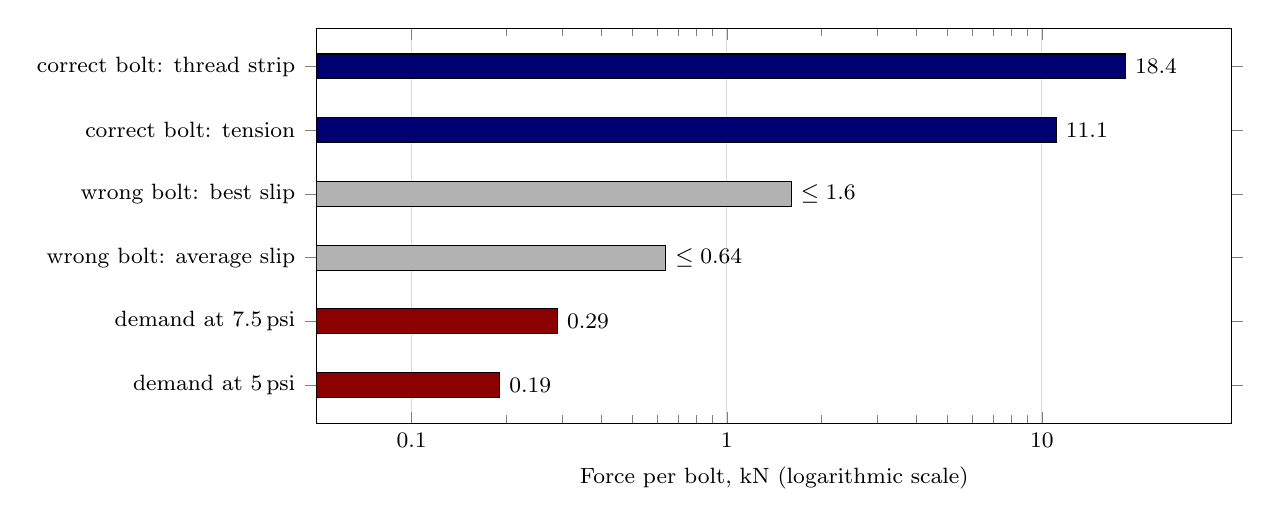
\begin{tikzpicture}
\begin{axis}[xbar,xmode=log,log origin=infty,width=13.2cm,height=6.6cm,xmin=0.05,xmax=40,
  bar width=9pt,bar shift=0pt,enlarge y limits=0.12,
  xlabel={Force per bolt, kN (logarithmic scale)},
  ytick={1,2,3,4,5,6},
  yticklabels={{demand at \SI{5}{psi}},{demand at \SI{7.5}{psi}},{wrong bolt: average slip},{wrong bolt: best slip},{correct bolt: tension},{correct bolt: thread strip}},
  yticklabel style={font=\footnotesize,align=right},xticklabel style={font=\footnotesize},xlabel style={font=\footnotesize},
  xtick={0.1,1,10},xticklabels={0.1,1,10},
  nodes near coords,nodes near coords style={font=\footnotesize,anchor=west},point meta=explicit symbolic,
  xmajorgrids,grid style={black!15}]
\addplot[fill=red!55!black,draw=black] coordinates {(0.19,1)[0.19] (0.29,2)[0.29]};
\addplot[fill=black!30,draw=black] coordinates {(0.64,3)[$\le0.64$] (1.6,4)[$\le1.6$]};
\addplot[fill=blue!45!black,draw=black] coordinates {(11.1,5)[11.1] (18.4,6)[18.4]};
\end{axis}
\end{tikzpicture}

\caption{Capacity and demand per bolt. The scale is logarithmic: the correct joint sits nearly two
decades above the load, the joint that was built sits on top of it. The wrong-bolt bars are upper
bounds from the slip tests.}
\label{fig:margin}
\end{figure}

\begin{center}\small
\begin{tabular}{@{}llll@{}}
\toprule
Case & Capacity per bolt & Demand per bolt & Capacity / demand\\
\midrule
A211-8D, bolt tension & \SI{11.1}{kN} & \SI{0.19}{kN} & about 58\\
A211-8C, average slip test & at most \SI{0.64}{kN} & \SI{0.19}{kN} & about 3\\
A211-8C, slipped at installation & near zero & \SI{0.19}{kN} & below 1\\
\bottomrule
\end{tabular}
\end{center}

\begin{keybox}{Why an average of three is not a margin of three}
Ninety bolts whose individual strengths run from nothing to a few hundred pounds do not share load
like ninety equal bolts. The weakest let go first; their neighbours pick up the load \emph{and} a
peeling moment as the screen lifts; the next weakest go; and the joint unzips around the frame.
Lecture 6 made the same point about a row of fasteners in shear --- they do not share equally ---
and it is truer still here. \textbf{The strength of a joint with scatter is set by its worst
fasteners, not its mean.}
\end{keybox}

\section{How the error got through}

The AAIB's findings are about people and organisations, and they are worth reading as an engineer,
because each one is a barrier that a designer or a procedure could have supplied.

\begin{enumerate}[leftmargin=*,itemsep=3pt]
\item \textbf{Part selection.} The Shift Maintenance Manager did not consult the Illustrated Parts
  Catalogue. He took a removed bolt to the stores and matched it by eye and by feel. The correct
  drawer held four or five bolts against a minimum stock of fifty, so he went to an unsupervised
  parts carousel in a poorly lit area and matched again by comparison. He needed mild glasses for
  small detail and was not wearing them. The bolts carry no identifying mark once out of the
  packet.
\item \textbf{A warning that was not pressed.} The stores supervisor told him that A211-8D bolts
  were used on that windscreen. He did not insist, and the remark was not acted on.
\item \textbf{Torque.} \SI{20}{lbf.in} instead of 15, with a screwdriver that was outside its
  calibration date. In the investigators' trials the tool's own residual friction was about
  \SI{30}{\percent} of the setting, against a normal 5 to \SI{10}{\percent}.
\item \textbf{The cue that was seen and misread.} The smaller heads did not fill the countersinks.
  He remembered afterwards that the countersinks had looked too big --- and had read that as an
  oversize countersink, not an undersize bolt. The evidence was in front of him; the wrong
  hypothesis absorbed it.
\item \textbf{No second pair of eyes, and no test.} The task was not classified as a ``Vital
  Point'', so no duplicate inspection was required, and nothing called for a pressure check before
  flight. In the report's words he ``had no backstop with any chance of detecting his errors.''
\item \textbf{Fatigue.} It was his first night shift after about five weeks; he had slept about an
  hour and a half beforehand, and the job was done between three and five in the morning.
\item \textbf{The organisation.} Quality audits and product samples did not watch how shift
  managers actually worked, so long-standing shortcuts were never seen.
\end{enumerate}

\noindent None of this was peculiar to one man or one night. When British Airways checked its
fleet by pulling every fourth bolt from the forward windscreens, two more aircraft failed and 41
short bolts were found; another operator found 107 on two of four aircraft (1.16).

\section{Lessons for joint design}

\begin{sumbox}{What to take from this into your own design work}
\begin{enumerate}[leftmargin=*,itemsep=2pt]
\item \textbf{Check thread stripping separately from bolt tension.} A sound design puts strip
  capacity above tensile capacity. That order depends on fit and engaged length --- on the pair ---
  and it is the first thing to go when the wrong part is fitted.
\item \textbf{Torque does not verify fit, and it does not verify preload.} It measures resistance
  to turning. A stripped thread and a released clutch feel alike at low torque.
\item \textbf{Keep fasteners out of the primary load path where you can.} A plug-type windscreen
  makes the same maintenance error harmless. This is the cheapest lesson on the page and it has to
  be learned at the drawing board; nobody can retrofit it in a hangar at four in the morning.
\item \textbf{Mistake-proof look-alike fasteners.} Two bolts with the same pitch, head and length
  that differ by \SI{0.026}{in} in diameter \emph{will} be confused. If two parts must not be
  interchanged, make them unable to be: a different pitch, a different drive, a different head, a
  kit supplied with the screen.
\item \textbf{A large static margin does not protect against the wrong part.} The margin of 58
  belonged to a joint that was not the one built. Margins cover scatter in loads and material;
  they do not cover a different design.
\item \textbf{If a joint cannot be inspected for correctness, test it before it carries people.}
  A ground pressurisation check would have found this.
\end{enumerate}
\end{sumbox}

\section{Questions to think about}

\begin{enumerate}[leftmargin=*,itemsep=3pt]
\item Repeat Step 1 at the \SI{7.5}{psi} design differential. How does capacity over demand change
  for the wrong bolts, and what does that say about \emph{when} in the flight this joint was always
  going to fail?
\item Six A211-7D bolts had the correct thread. Could they alone have held the windscreen?
  Consider their reduced engagement, where on the frame they were, and peel.
\item Recalculate the strip area for the correct pair at minimum-material limits (bolt pitch
  diameter \SI{0.1658}{in}, nut minor diameter \SI{0.164}{in}) instead of basic sizes. Does the
  bolt still fail before the thread?
\item The engineer applied \SI{20}{lbf.in} against a specified 15. For the \emph{correct} bolt,
  calculate the preload at each and the fraction of proof load. Was the overtorque itself
  dangerous? What does your answer tell you about which of his errors mattered?
\item You are asked to redesign the fastener so that an 8-32 bolt cannot be fitted in this
  position. Propose two different ways, and for each say what it costs the operator.
\item Which single change would you make first: the design, the fastener standard, or the
  inspection procedure? Defend the choice in five sentences.
\end{enumerate}

\section*{Sources}

\begin{itemize}[leftmargin=*,itemsep=1pt,font=\footnotesize]
\item[] {\footnotesize Air Accidents Investigation Branch, \emph{Report on the accident to BAC
  One-Eleven, G-BJRT, over Didcot, Oxfordshire, on 10 June 1990}, Aircraft Accident Report 1/92.
  Source of the bolt part numbers, counts and measured diameters (1.12.1), the windscreen
  installation and the quotation on bolt numbers (1.6.3), the thread-slip trials (1.16.1), the
  torque values and stores details (1.17.4), the shift and sleep details (1.17.6), and the causal
  factors (section 3).}
\item[] {\footnotesize Thread dimensions and tensile stress areas: Unified thread standard values
  as tabulated in Shigley, Table 8-2. Strip-area formula: FED-STD-H28; see also Bickford,
  \emph{Introduction to the Design and Behavior of Bolted Joints}.}
\end{itemize}

\vspace{4pt}
\noindent{\footnotesize\emph{Note on the arithmetic.} The load, capacity and margin figures in
\S\ref{sec:arith} are worked in this handout. The cabin differential, windscreen area, bolt
strength, engaged length and nut factor are assumptions made for teaching and are marked as such;
they are not report data. The slip torques are the investigation's; their conversion to force is
ours.}

\end{document}
